\documentclass{article}
\usepackage{tikz}

\begin{document}
    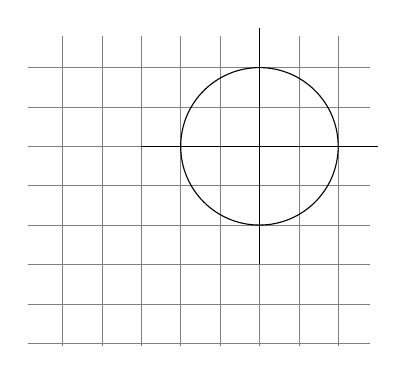
\begin{tikzpicture}
        \draw[step=.5cm, gray, very thin] (-1.4, -1,4) grid (1.4, 1.4);
        \draw (-1.5, 0) -- (1.5, 0);
        \draw (0, -1.5) -- (0, 1.5);
        \draw (0, 0) circle[radius=1cm];
    \end{tikzpicture}
    \newpage
    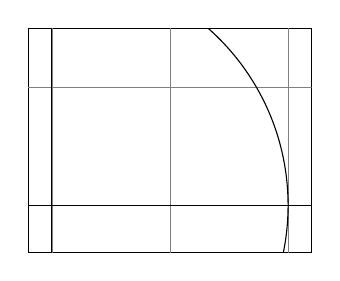
\begin{tikzpicture}[scale=3]
        \clip[draw] (-0.1, -0.2) rectangle (1.1, 0.75);
        \draw[step=.5cm, gray, very thin] (-1.4, -1,4) grid (1.4, 1.4);
        \draw (-1.5, 0) -- (1.5, 0);
        \draw (0, -1.5) -- (0, 1.5);
        \draw (0, 0) circle[radius=1cm];
    \end{tikzpicture}
    \newpage
    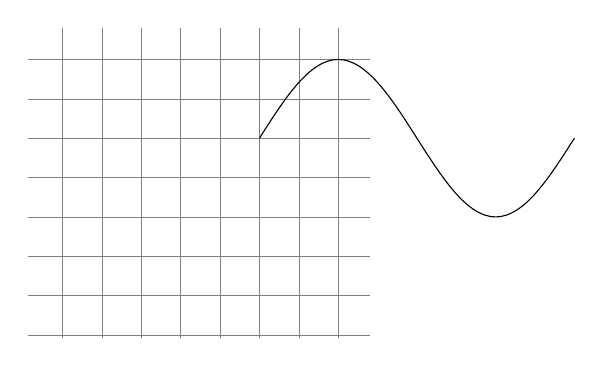
\begin{tikzpicture}
        \draw[step=.5cm, gray, very thin] (-1.4, -1,4) grid (1.4, 1.4);
        \draw (0, 0) sin (1, 1) cos (2, 0) sin (3, -1) cos (4, 0);
    \end{tikzpicture}
\end{document}